% An original rendering of boundary status as a set of tracks.
%
% Deliberately NOT the familiar radial wheel. Each regulating system is a track
% running left to right from the safe range, through a band of increasing risk,
% into a zone of high risk. A marker gives where the framework judged the system
% to sit. Position is qualitative on purpose: the point of the diagram is the
% structure of the assessment, and not a set of values to be read off.
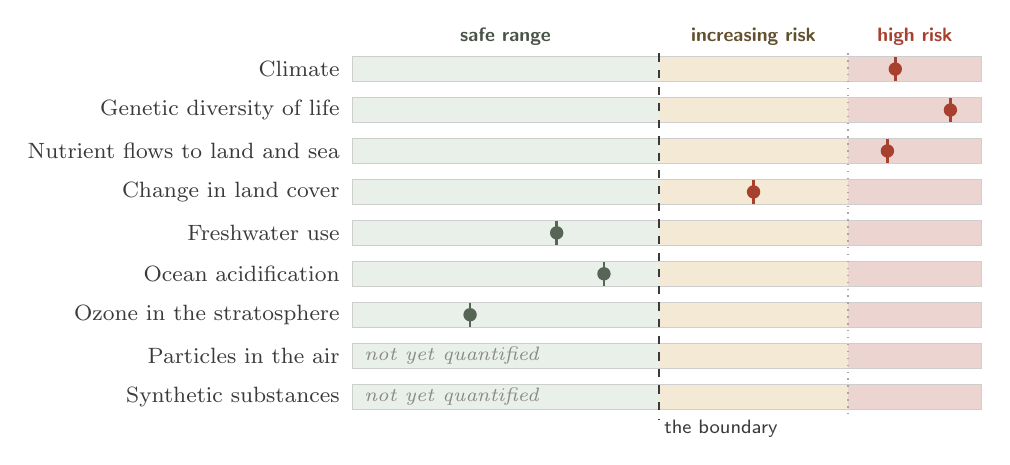
\begin{tikzpicture}[
  font=\footnotesize,
  every node/.style={inner sep=0pt},
]

\definecolor{zsafe}{HTML}{9CB89A}
\definecolor{zrisk}{HTML}{D9B166}
\definecolor{zhigh}{HTML}{A8402F}
\definecolor{ink}{HTML}{3A3A3A}

\def\L{0}      % left of track
\def\A{3.9}    % end of safe
\def\B{6.3}    % end of increasing risk
\def\R{8.0}    % right end
\def\dy{0.52}

% zone headers
\node[anchor=south, text=zsafe!45!black, font=\scriptsize\sffamily\bfseries]
  at ({(\L+\A)/2},{0.30}) {safe range};
\node[anchor=south, text=zrisk!45!black, font=\scriptsize\sffamily\bfseries]
  at ({(\A+\B)/2},{0.30}) {increasing risk};
\node[anchor=south, text=zhigh, font=\scriptsize\sffamily\bfseries]
  at ({(\B+\R)/2},{0.30}) {high risk};

\def\rows{%
  {Climate}/{6.9}/1,
  {Genetic diversity of life}/{7.6}/1,
  {Nutrient flows to land and sea}/{6.8}/1,
  {Change in land cover}/{5.1}/1,
  {Freshwater use}/{2.6}/0,
  {Ocean acidification}/{3.2}/0,
  {Ozone in the stratosphere}/{1.5}/0,
  {Particles in the air}/{-1}/2,
  {Synthetic substances}/{-1}/2%
}

\foreach \name/\pos/\state [count=\i from 0] in \rows {
  \pgfmathsetmacro{\y}{-\i*\dy}
  % zones
  \fill[zsafe!22] (\L,\y-0.16) rectangle (\A,\y+0.16);
  \fill[zrisk!28] (\A,\y-0.16) rectangle (\B,\y+0.16);
  \fill[zhigh!22] (\B,\y-0.16) rectangle (\R,\y+0.16);
  \draw[ink!25, line width=0.3pt] (\L,\y-0.16) rectangle (\R,\y+0.16);
  % label
  \node[anchor=east, text=ink] at (\L-0.15,\y) {\name};
  % marker
  \ifnum\state=2
    \node[anchor=west, font=\scriptsize\itshape, text=ink!60]
      at (\L+0.15,\y) {not yet quantified};
  \else
    \ifnum\state=1
      \fill[zhigh] (\pos,\y) circle (0.085);
      \draw[zhigh, line width=0.9pt] (\pos,\y-0.15) -- (\pos,\y+0.15);
    \else
      \fill[zsafe!55!black] (\pos,\y) circle (0.085);
      \draw[zsafe!55!black, line width=0.9pt] (\pos,\y-0.15) -- (\pos,\y+0.15);
    \fi
  \fi
}

% the boundary line itself
\draw[ink, line width=0.8pt, dashed]
  (\A,0.20) -- (\A,{-8*\dy-0.28});
\node[anchor=south west, font=\scriptsize\sffamily, text=ink]
  at (\A+0.06,{-8*\dy-0.52}) {the boundary};

\draw[ink!45, line width=0.5pt, dotted]
  (\B,0.20) -- (\B,{-8*\dy-0.28});

\end{tikzpicture}
